%-------------------------------
%	PACKAGES AND OTHER DOCUMENT CONFIGURATIONS
%-------------------------------

% The \vref command specifies the location of the reference

%\documentclass[
%10pt, % Main document font size
%a4paper, % Paper type, use 'letterpaper' for US Letter paper
%oneside, % One page layout (no page indentation)
%twoside, % Two page layout (page indentation for binding and different headers)
%headinclude,footinclude, % Extra spacing for the header and footer
%BCOR5mm, % Binding correction
%]{scrartcl}


\documentclass{article}


%--------------------------------------------------------------
%	REQUIRED PACKAGES
%--------------------------------------------------------------

\usepackage[
nochapters, % Turn off chapters since this is an article        
beramono, % Use the Bera Mono font for monospaced text (\texttt)
%eulermath,% Use the Euler font for mathematics
pdfspacing, % Makes use of pdftex’ letter spacing capabilities via the microtype package
dottedtoc % Dotted lines leading to the page numbers in the table of contents
]{classicthesis} % The layout is based on the Classic Thesis style



\usepackage{arsclassica} % Modifies the Classic Thesis package

\usepackage[T1]{fontenc} % Use 8-bit encoding that has 256 glyphs

\usepackage[utf8]{inputenc} % Required for including letters with accents
%--------------------------------------------------------------
% Fonts and languages
\usepackage{libertinus} % The Libertinus font
%\usepackage[adobe-utopia]{mathdesign} % The Utopia font
%\usepackage[p,osf]{scholax}
% T1 and textcomp are loaded by package. Change that here, if you want
% load sans and typewriter packages here, if needed
%\usepackage{amsmath,amsthm}% must be loaded before newtxmath
% amssymb should not be loaded
%\usepackage[scaled=1.075,ncf,vvarbb]{newtxmath}% need to scale up math package
% vvarbb selects the STIX version of blackboard bold.


\usepackage[czech]{babel} % Český jazyk
%--------------------------------------------------------------
\usepackage{graphicx} % Required for including images
\graphicspath{{Figures/}} % Set the default folder for images

\usepackage{enumitem} % Required for manipulating the whitespace between and within lists

\usepackage{lipsum} % Used for inserting dummy 'Lorem ipsum' text into the template

\usepackage{subfig} % Required for creating figures with multiple parts (subfigures)

\usepackage{amsmath,amssymb,amsthm,amsfonts} % For including math equations, theorems, symbols, etc

\usepackage{varioref} % More descriptive referencing

\usepackage[top =3 cm, bottom = 3.5 cm, left = 1.5 cm, right = 1.5 cm]{geometry}

\usepackage{mathtools}

\usepackage{float}

\usepackage{caption}

%------------------------------------------------------------
%	DIAGRAMS AND TIKZ
\usepackage{smartdiagram}
\usepackage{metalogo}
\usepackage{tikz}
\usetikzlibrary{matrix,calc}

\usepackage{hhline} % kvůli double line v tabulkách
%------------------------------------------------------------
%	THEOREM STYLES
%------------------------------------------------------------

\theoremstyle{definition} % Define theorem styles here based on the definition style (used for definitions and examples)
\newtheorem{definition}{Definice}
\newtheorem{example}{Příklad}
\newtheorem{exercise}{Cvičení}

\theoremstyle{plain} % Define theorem styles here based on the plain style (used for theorems, lemmas, propositions)
\newtheorem{theorem}{Věta}

\theoremstyle{remark} % Define theorem styles here based on the remark style (used for remarks and notes)
\newtheorem{remark}{Poznámka}



%-------------------------------------------------------------
%	HYPERLINKS
%-------------------------------------------------------------

\hypersetup{
%draft, % Uncomment to remove all links (useful for printing in black and white)
colorlinks=true, breaklinks=true, bookmarks=true,bookmarksnumbered,
urlcolor=webbrown, linkcolor=RoyalBlue, citecolor=webgreen, % Link colors
pdftitle={}, % PDF title
pdfauthor={\textcopyright}, % PDF Author
pdfsubject={}, % PDF Subject
pdfkeywords={}, % PDF Keywords
pdfcreator={pdfLaTeX}, % PDF Creator
pdfproducer={LaTeX with hyperref and ClassicThesis} % PDF producer
}

 % Include the structure.tex file which specified the document structure and layout

%----------------------------------------------------
%	MATHEMATICS
%----------------------------------------------------

% Tělesa, obory íntegrity a metrické prostory
\newcommand{\C}{\mathbb{C}}
\newcommand{\R}{\mathbb{R}}
\newcommand{\N}{\mathbb{N}}
\newcommand{\Q}{\mathbb{Q}}
\newcommand{\Z}{\mathbb{Z}}
\renewcommand{\L}[2]{L^{#1} \left( #2 \right)} % Lebesgueovy prostory

\newcommand{\vc}[1]{\boldsymbol{#1}} % vektor
\newcommand{\mat}[1]{\mathbf{#1}} % matice

\newcommand{\norm}[1]{\left \Vert #1 \right \Vert} % norma vektoru
\newcommand{\set}[1]{ \left \lbrace #1 \right \rbrace} % množina
\newcommand{\const}{\mathrm{konst}} % konstanta

\newcommand{\F}{\mathcal{F} } % Fourierova transformace
\newcommand{\La}{\mathcal{L}} % Laplaceova transformace

% Označení funkcí
\newcommand{\Res}[2]{\mathrm{Res}_{#1} \, #2 \,} % residuum
\newcommand{\sgn}{\, \mathrm{sign} \,} % signum
\newcommand{\tg}{\,\mathrm{tg}\,} % možné značení tangens


%Značení derivací a integrálů
\newcommand{\der}[2]{\frac{\mathrm{d}#1}{\mathrm{d}#2}} % obyčejná derivace
\newcommand{\pder}[2]{\frac{\partial #1}{\partial #2}} % parciální derivace
\newcommand{\tder}[3]{\left( \pder{#1}{#2} \right)_{#3 = \const}} % termodynamická derivace
\newcommand{\D}{\mathrm{d} } % integrační znamení
\newcommand{\DD}{\mathrm{D}} % absolutní derivace
\newcommand{\intR}{\int_{-\infty}^{\infty}} % integrál přes reálnou osu



% Značení posloupností, limit a sum
\newcommand{\sequence}[2]{ \left \lbrace #1 \right \rbrace_{#2=1}^\infty} % posloupnost
\newcommand{\sumnorm}[1]{\sum_{#1}^\infty} 
\newcommand{\limplus}[1]{\lim_{#1 \rightarrow + \infty}}
\newcommand{\limminus}[1]{\lim_{#1 \rightarrow - \infty}}


% VŠE záležitosti
\newcommand{\dder}[2]{\frac{\Delta #1}{\Delta #2}}


\newcommand{\arctg}{\mathrm{arctg}\,}
\newcommand{\cotg}{\mathrm{cotg}\,}
\newcommand{\arccotg}{\mathrm{arccotg}\,} % Include the mathematics.tex file which uses some mathematical operators

\hyphenation{Fortran hy-phen-ation} % Specify custom hyphenation points in words with dashes where you would like hyphenation to occur, or alternatively, don't put any dashes in a word to stop hyphenation altogether

%-------------------------------
%	TITLE AND AUTHOR(S)
%-------------------------------

%\title{\normalfont\spacedallcaps{Article Title}} % The article title

%\subtitle{Subtitle} % Uncomment to display a subtitle

\author{\spacedlowsmallcaps{Miroslav Burýšek*}} % The article author(s) - author affiliations need to be specified in the AUTHOR AFFILIATIONS block

\date{\today} % An optional date to appear under the author(s)




%-------------------------------------
%	TESTING
%-------------------------------------
% Load packages for testing
\usepackage{blindtext}
%\usepackage{showframe} % Uncomment to show boxes around the text area, margin, header and footer
%\usepackage[inline]{showlabels}  \showlabels[\small\color{JungleGreen}]{}  % Uncomment to output the content of \label commands to the document where they are used


\begin{document}

%-------------------------------------------
%	HEADERS
%-------------------------------------------

\renewcommand{\sectionmark}[1]{\markright{\spacedlowsmallcaps{#1}}} % The header for all pages (oneside) or for even pages (twoside)
%\renewcommand{\subsectionmark}[1]{\markright{\thesubsection~#1}} % Uncomment when using the twoside option - this modifies the header on odd pages
\lehead{\mbox{\llap{\small\thepage\kern1em\color{halfgray} \vline}\color{halfgray}\hspace{0.5em}\rightmark\hfil}} % The header style

\pagestyle{scrheadings} % Enable the headers specified in this block





%-----------------------------------------
%	TABLE OF CONTENTS & LISTS OF FIGURES AND TABLES
%-----------------------------------------

%\maketitle % Print the title/author/date block

\setcounter{tocdepth}{2} % Set the depth of the table of contents to show sections and subsections only

%\tableofcontents % Print the table of contents

%\listoffigures % Print the list of figures

%\listoftables % Print the list of tables






%--------------------------------------
%	ABSTRACT
%--------------------------------------

%\section*{Abstract} % This section will not appear in the table of contents due to the star (\section*)


%---------------------------------------
%	AUTHOR AFFILIATIONS
%---------------------------------------

\let\thefootnote\relax\footnotetext{\textbf{Verze:} \today }

%--------------------------------------

%\newpage % Start the article content on the second page, remove this if you have a longer abstract that goes onto the second page

%\section*{Definiční obory elementárních funkcí}

Při určování definičního oboru elementárních funkcí se v podstatě můžeme řídit jednoduchými zásadami.

\begin{enumerate}
    \item Nesmíme dělit nulou.
    \item Sudé odmocniny jsou definované pouze pro nezáporná čísla.
    \item Logaritmus je definovaný pouze pro kladná čísla.
    \item Speciální pozornost si zaslouží funkce $\tg x$, $\cotg x$, $\arcsin x $ a $\arccos x$.
\end{enumerate}

Kompletní přehled dává tabulka \ref{tab:funkce}. (Je víceméně potřeba umět ji nazpaměť.)

\begin{table}[H]
    \centering
    \begin{tabular}{|c|c|c|}
        \hline
        \textbf{funkce} & \textbf{definiční obor} & \textbf{obor hodnot} \\
        \hline
        $x^k$, $k$ je sudé              & $\R$          & $[0, \infty)$ \\ 
        $x^k$, $k$ je liché             & $\R$          & $\R$ \\ 
        $\sqrt[k]{x}$, $k$ je sudé      & $[0, \infty)$ & $[0, \infty)$ \\
        $\sqrt[k]{x}$, $k$ je liché     & $\R$          & $\R$ \\
        \hline
        $e^x$                           & $\R$          & $(0, \infty)$ \\
        $a^x$, $a>0$                    & $\R$          & $(0, \infty)$ \\
        $\ln x$                         & $(0, \infty)$ & $\R$ \\
        $\log_a x$, $a>0$               & $(0, \infty)$ & $\R$ \\
        \hline
        $\sin x$                        & $\R$          & $[0,1]$ \\
        $\cos x$                        & $\R$          & $[0,1]$ \\
        $\tg x$                         & $\R \setminus \set{\pi/2 + k \pi, k \in \Z}$ & $\R$ \\
        $\cotg x$                       & $\R \setminus \set{k \pi, k \in \Z}$  & $\R$ \\
        \hline
        $\arcsin x$                     & $[-1,1]$      & $[-\frac{\pi}{2}, \frac{\pi}{2}]$ \\
        $\arccos x$                     & $[-1,1]$      & $[0,\pi]$ \\
        $\arctg x$                      & $\R$          & $(-\frac{\pi}{2}, \frac{\pi}{2})$ \\
        $\arccotg x$                    & $\R$          & $(0,\pi)$ \\
         \hline
    \end{tabular}
    \caption{Tabulka elementárních funkcí.}
    \label{tab:funkce}
\end{table}

\section*{Příklady}

\begin{example}
    Určíme definiční obor funkce \begin{align}
        f(x) = \frac{1}{x-4} + \frac{1}{x+6} \:.
    \end{align}
    P1 nám říká, že nesmíme dělit nulou. To vede na podmínky $x \neq 4$ a $x \neq -6$. To jsou body, které musíme vyřadit z množiny reálných čísel, abychom získali definiční obor. Množinově to lze zapsat jako 
    \begin{align}
        D_f = \R \setminus \set{4,-6} \:,
    \end{align}
    kde symbol \uv{$\setminus$} značí množinový rozdíl. To samé můžeme napsat pomocí sjednocení intervalů 
    \begin{align}
        D_f = (-\infty,-6) \cup (-6,4) \cup (4,+\infty) \:.
    \end{align}
    Kulaté závorky značí otevřené intervaly, to znamená, že do nich krajní body nepatří.
\end{example}


\begin{example}
    Určíme definiční obor funkce \begin{align}
        g(x) = \frac{(x-2)(x-6)}{(x-4)(x^2-9)} \:.
    \end{align}
    Použijeme opět P1 a dostáváme rovnici \begin{align}
        (x-4)(x^2-9) = 0 \:.
    \end{align}
    Nyní využijeme toho, že \textit{součin čísel je roven nule právě tehdy, když alespoň jedno z nich je rovno nule}. Dostáváme tedy podmínky:
    \begin{align}
        x - 4 = 0 \implies x \neq 4 \\
        x^2 - 9 = 0 \implies x \neq \pm 3 \:.
    \end{align}
    Celkově $D_g = \R \setminus \set{-3,3,4}$.
\end{example}

\begin{example}
    Určíme definiční obor funkce \begin{align}
        h(x) = \sqrt{1 - \frac{6}{x+1}} \:.
    \end{align}
    P1 nám dává podmínku $x \neq -1$. P2 nám říká, že celý výraz pod odmocninou musí být nezáporný, tedy \begin{align}
        1 - \frac{6}{x+1} \geq 0 \:.
    \end{align}
    Tuto nerovnici můžeme vyřešit například tak, že převedeme oba členy na stejného jmenovatele
    \begin{align}
        \frac{x+1}{x+1} - \frac{6}{x+1} = \frac{x-5}{x+1} \geq 0
    \end{align}
    a poté využijeme toho, že \textit{podíl dvou čísel je nezáporný tehdy, když čitatel i jmenovatel budou buďto oba dva kladné nebo oba dva záporné}. Samozřejmě ale musíme vyloučit možnost $x=-1$. Takže \begin{align}
        [x-5 \leq 0] \bigwedge [x+1 > 0] \implies x \in [5,\infty) \\
        [x-5 \geq 0] \bigwedge [x+1 < 0] \implies x \in (-\infty,-1) 
    \end{align}
    Celkově $D_h = (-\infty, -1) \cup [5,\infty)$.
\end{example}

\begin{example}
    Určíme definiční obor funkce \begin{align}
        F(x) = \frac{\sqrt{4-\ln x}}{2^x - 16} \:.
    \end{align}
    P1 vede na rovnici $2^x - 16 = 0$. Tu můžeme snadno vyřešit, když si všimneme, že $16 = 2^4$, takže $x \neq 4$.
    P3 vede na podmínku $x>0$. Konečně P2 vede na nerovnici \begin{align}
        4 - \ln x \geq 0 \:.
    \end{align}
    Tu můžeme vyřešit tak, že logaritmus převedeme na jednu stranu rovnice
    \begin{align}
        4 \geq \ln x \:.
    \end{align}
    Nyní můžeme na rovnici \uv{zapůsobit exponenciálou}. Exponenciála je funkce prostá a rostoucí, nemění se tedy znaménko nerovnosti. Dostáváme \begin{align}
        \exp(4) = e^4 \geq \exp(\ln x) = x \:,
    \end{align}
    takže $x \in (-\infty, e^4]$.
    
    Celkově dostáváme $D_F = (0,4)\cup(4,e^4]$.
\end{example}

\begin{example}
    Určíme definiční obor funkce \begin{align}
        G(t) = \arcsin (\ln t) \:.
    \end{align}
    P3 nám říká, že $t>0$. Nyní se podíváme na pravidlo P4. To nám říká, že argument (\uv{vnitřek}) arkussinu musí být v mezích $[-1,1]$. Odtud dostáváme podmínku \begin{align}
        -1 \leq \ln t \leq +1 \:.
    \end{align}
    Tyto nerovnice můžeme vyřešit opět tak, že zapůsobíme exponenciálou:
    \begin{align}
        e^{-1} \leq t \leq e^1 \:.
    \end{align}
    Celkově tedy $D_G = [e^{-1},e]$.
\end{example}

\begin{example}
    Určíme definiční obor funkce \begin{align}
        y(x) = \ln \left( \frac{\pi}{6} - \arcsin x \right) \:.
    \end{align}
    P4 nám říká, že $x \in [-1,1]$. P3 nám dává nerovnici \begin{align}
        \frac{\pi}{6} - \arcsin x > 0 \:.
    \end{align}
    Takovou nerovnici opět vyřešíme tak, že arkussinus převedeme na druhou stranu rovnice
    \begin{align}
        \frac{\pi}{6} > \arcsin x
    \end{align}
    a na rovnici \uv{zapůsobíme} funkcí sinus. Ta je opět rostoucí, takže nezmění znaménko nerovnosti. Dostáváme
    \begin{align}
        \frac{1}{2} = \sin \left( \frac{\pi}{6} \right)  > \sin (\arcsin(x)) = x \:,
    \end{align}
    takže máme $x \in (-\infty, \frac{1}{2})$.

    Celkově $D_y = [-1,\frac{1}{2})$.
\end{example}

\begin{example}[Náročnější]
    Určíme definiční obor funkce \begin{align}
        T(z) = \ln \left(\ln(\ln z) \right) \:.
    \end{align}
    Aplikujeme pravidlo P3, postupovat budeme od funkce uvnitř. Dostaneme podmínky \begin{align}
        z > 0 \:, \quad \ln (z) > 0 \:, \quad \ln (\ln z) > 0 \:.
    \end{align}
    Druhá z nerovnic nám dává podmínku $z > 1$. Na třetí nerovnici aplikujeme exponenciálu a dostaneme \begin{align}
        \ln z > \exp 0 = 1 \:.
    \end{align}
    Nyní znova zapůsobíme exponenciálou a dostaneme \begin{align}
        z >  \exp 1 = e \:.
    \end{align}

    Takže $D_T = (e, \infty)$.
\end{example}

\begin{example}[S absolutní hodnotou]
    Určíme definiční obor funkce \begin{align}
        A(x) = \frac{1}{\sqrt{|x+2|-|x+4|}} \:.
    \end{align}
    P1 a P2 vedou na podmínku \begin{align}
        |x+2|-|x+4| > 0 \:.
    \end{align}
    Absolutních hodnot se zbavíme tak, že se podíváme na jednotlivé intervaly. Nulové body v absolutních hodnotách jsou $-2$ a $-4$. Dostáváme tak tři intervaly, na kterých budeme absolutní hodnoty řešit:
    \begin{table}[H]
        \centering
        \begin{tabular}{c|c|c|c}
            interval & $(-\infty,-4) $ & $(-4,-2)$ & $(-2,\infty)$ \\
            \hline
            $|x+2|$ & $-x-2$ & $-x-2$ & $x+2$ \\
            $|x+4|$ & $-x-4$ & $x+4$ & $x+4$ \\
            \hline
            $|x+2|-|x+4|$ & $(-x-2)-(-x-4)=2$ & $(-x-2)-(x+4)=-2x-6$ & $(x+2)-(x+4) = -2$
        \end{tabular}
    \end{table}
    Na intervalu $(-\infty,-4)$ se tedy suma absolutních hodnot chová jako konstanta $2$, která je zřejmě větší než nula. 
    
    Na intervalu $(-4,-2)$ musíme vyřešit nerovnici $-2x-6>0$, která vede na $x < -3$. 
    
    Na intervalu $(-2,\infty)$ už je chování zase konstantní, $-2<0$. 
    
    Celkově vyhovují pouze $x$ z intervalu $(-\infty,-4]$ a ještě z intervalu $[-4,-3)$. Takže $D_A = (-\infty,-3)$.
\end{example}

\subsection*{Závěrečné poznámky}

\begin{itemize}
    \item Časté chyby, na které je dobré dát zvláštní pozor:
    \begin{itemize}
        \item Záporná mocnina kladného čísla je stále kladné číslo! Například $2^{-4} = \frac{1}{2^4} = \frac{1}{16} > 0$.\newline To je rozdíl oproti $2^{-4} \neq -2^4 = -16$!
        \item Násobíme-li nerovnici záporným číslem, obrací se znaménko nerovnosti! Například nerovnici $-2x^2 > -4x$ můžeme vydělit $-2$ a dostaneme $x^2 < 2x$.
        \item Definiční obor musíme určit z původního výrazu, ještě předtím, než ho začneme dále upravovat. Tak například funkce \begin{align}
            f(x) = 1 \:, \quad g(x) = \frac{x(x+1)}{x(x+1)}
        \end{align}
        dávají pro všechna přípustná $x$ stejné hodnoty, ale definiční obor funkcí je různý! \newline $D_f = \R$, zatímco $D_g = \R \setminus \set{0,-1}$.
    \end{itemize}

\end{itemize}

%\section{Vektory}

Uspořádanou $n$-tici reálných čísel $\vc v = (v_1,v_2,v_3, \cdots, v_n)$ budeme nazývat \textbf{vektorem} délky $n$. Množinu všech vektorů délky $n$ budeme značit $V_n$ a nazývat ji \textbf{vektorovým prostorem}. Číslu $a_j$ na $j$-té pozici ve vektoru $\vc a$ říkáme \textbf{$j$-tá složka vektoru}.

Definujeme součet vektorů (po složkách) \begin{align}
    (a_1,a_2,\cdots, a_n) + (b_1,b_2,\cdots, b_n) = (a_1+b_1, a_2 + b_2, \cdots , a_n + b_n)
\end{align}
a násobek vektoru reálným číslem (rovněž po složkách) \begin{align}
    c (a_1, a_2, \cdots, a_n) = (c a_1, c a_2, \cdots, c a_n) \:.
\end{align}
Je jasné, že sčítat lze pouze dva vektory stejné délky.

\begin{example}
    Nechť $\vc x = (1,-2,4,6)$, $\vc y = (1,0,0,2)$ a $\vc z = (2,-1,1)$. Platí \begin{align}
        \vc x - 3 \vc y = (1,-2,4,6) - 3\cdot(1,0,0,2) = (1-3,-2,4,6-6) = (-2,-2,4,0) \:.
    \end{align}
    Vektor $\vc z$ nemůžeme sčítat s vektory $\vc x$ a $\vc y$, protože $\vc z \in V_3$, ale $\vc x, \vc y \in V_4$.
\end{example}

\subsection*{Příklady použití vektorů}

\begin{itemize}
    \item Prostor $V_1$ je složen z vektorů délky $1$, tedy z objektů typu $ \vc a = (a)$. Je tedy v nějakém smyslu totožný, jako množina reálných čísel $\R$.
    \item Prostor $V_2$ je složen z vektorů délky $2$, které mohou reprezentovat například aritmetické vektory v rovině, známé z analytické geometrie. Tam se většinou značí se šipkou:
    \begin{align}
        \overrightarrow{v} = (v_x,v_y) \:.
    \end{align}
    \item Prostor $V_3$ z vektorů délky $3$, které mohou reprezentovat aritmetické vektory v prostorové třírozměrné geometrii. Také se často značí se šipkou:
    \begin{align}
        \overrightarrow{v} = (v_x,v_y,v_z) \:.
    \end{align}
    \item Operace násobení vektoru číslem v prostorech $V_2$ a $V_3$ představuje \uv{natahování nebo zkracování vektoru}.
    \item V Newtonově pohybovém zákonu $\overrightarrow{F} = m \overrightarrow{a}$ vystupují vektory z $V_3$. $m$ je hmotnost objektu, $\overrightarrow{F}$ je působící síla a $\overrightarrow{a}$ je zrychlení objektu, které tato síla způsobí.
    \item Do vektoru délky $n$ můžeme ukládat například ceny jednotlivých výrobků, které máme seřazené podle nějakého kritéria.
\end{itemize}

\section{Lineární kombinace, lineární (ne)závislost}

Řekneme, že vektor $\vc x$ je \textbf{lineární kombinací} vektorů $\vc a_1, \vc a_2, \cdots, \vc a_k$, jestliže existují čísla $c_1, c_2, \cdots, c_n$ taková, že platí \begin{align}
    \vc x = c_1 \vc a_1 + c_2 \vc a_2 + \cdots + c_k \vc a_k \:.
\end{align}
Koeficientům $c_1, \cdots, c_k$ říkáme \textbf{koeficienty lineární kombinace}. 

Řekneme, že vektory $\vc a_1, \vc a_2, \cdots, \vc a_k$ jsou \textbf{lineárně závislé}, jestliže existuje jejich netriviální lineární kombinace nulového vektoru, tj. existují \underline{nenulová čísla} $c_1, c_2 \cdots, c_n$ taková, že \begin{align}
    \vc 0 = c_1 \vc a_1 + c_2 \vc a_2 + \cdots + c_k \vc a_k \:.
\end{align}
Jestliže vektory nejsou lineárně závislé, říkáme, že jsou \textbf{lineárně nezávislé}.

Zřejmě platí, že vektory $\vc a_1, \vc a_2, \cdots, \vc a_k$ jsou lineárně závislé právě tehdy, když je jeden z nich lineární kombinací ostatních. Nechť je to například vektor $\vc a_j$, takže ho lze vyjádřit vztahem \begin{align}
    \vc a_j = c_1 \vc a_1 + c_2 \vc a_2 + \cdots + c_{j-1} \vc a_{j-1} + c_{j+1} \vc a_{j+1} + \cdots + c_k \vc a_k \:.
\end{align}
Pak ho zřejmě můžeme od obou stran rovnice odečíst a dostáváme \begin{align}
    \vc 0 = c_1 \vc a_1 + c_2 \vc a_2 + \cdots + c_{j-1} \vc a_{j-1} - 1 \cdot \vc a_j + c_{j+1} \vc a_{j+1} + \cdots + c_k \vc a_k \:.
\end{align}
Tím jsme našli netriviální lineární kombinaci nuly, takže jsou vektory lineárně závislé. Úvaha funguje oběma směry.

\begin{example}
    Vektory $\vc a = (1,2,-4)$ a $\vc b = (-2,-4,8)$ jsou zřejmě lineárně závislé, protože je jeden lineární kombinací druhého: $-2 \vc a = \vc b$, takže
    \begin{align}
        \vc 0 = 2 \vc a + \vc b  \:.
    \end{align}

    Vektory $\vc a = (1,1,0)$ a $\vc b = (0,0,4)$ jsou lineárně nezávislé. Jediná možnost, jak z těchto vektorů \uv{poskládat} nulový vektor, je \begin{align}
        \vc 0 = 0 \cdot \vc a + 0 \cdot \vc b \:.
    \end{align}
\end{example}

\section{Matice}

Obdélníkové schéma reálných čísel typu \begin{align}
    \mat A = \begin{pmatrix}
        a_{11} & a_{12} & a_{13} & \cdots & a_{1n} \\
        a_{21} & a_{22} & a_{23} & \cdots & a_{2n} \\
        a_{31} & a_{32} & a_{33} & \cdots & a_{3n} \\
        \vdots & \vdots & \vdots & \ddots & \vdots \\
        a_{m1} & a_{m2} & a_{m3} & \cdots & a_{mn} 
    \end{pmatrix}
\end{align}
o $m$ řádcích a $n$ sloupcích nazýváme \textbf{maticí} typu $m \times n$.

Jednotlivé řádky, resp. sloupce mohou reprezentovat vektory. Můžeme se také dívat na vektory jako na matice typu $1 \times n$.

Sčítání matic a násobení matic reálným číslem definujeme stejně jako u vektorů po složkách:
\begin{align}
    c \mat A = \begin{pmatrix}
        c a_{11} & c a_{12}  & \cdots & c a_{1n} \\
        c a_{21} & c a_{22}  & \cdots & c a_{2n} \\
        \vdots & \vdots & \ddots & \vdots \\
        c a_{m1} & c a_{m2} & \cdots & c a_{mn} 
    \end{pmatrix} \:, 
    \quad 
    \mat A + \mat B = \begin{pmatrix}
        a_{11} + b_{11} & a_{12} + b_{21}  & \cdots & a_{1n}+ b_{1n} \\
        a_{21} + b_{21} & a_{22} + b_{22} & \cdots & a_{2n} + b_{2n}\\
        \vdots & \vdots & \ddots & \vdots \\
        a_{m1} + b_{m1} & a_{m2} + b_{m2} & \cdots & a_{mn} + b_{mn} 
    \end{pmatrix} \:.
\end{align}

\subsection*{Příklady použití matic}

\begin{itemize}
    \item Do matice typu $12 \times n$ můžeme uložit ceny jednotlivých výrobků během roku. Prvek matice $a_{ij}$ bude reprezentovat cenu $j$-tého výrobku v $i$-tém kalendářním měsíci.
    \item Stejně tak bychom mohli ukládat např. ceny akcií v jednotlivých dnech. Hospodářské přílohy novin nebo zpravodajské weby zveřejňují každý den nový řádek matice.
    \item Digitální fotoaparát zaznamenává každý pixel jako jeho barvu. Barva se skládá ze tří základních složek - RGB. Intenzitu každé jedné barvy zaznamenává číslo mezi $-127$ až $128$. Jedna fotka vyrobená fotoaparátem, který má $8$ Mpixelů by tak vyžadovala paměť $24$ MB, takže na disk o velikosti $1$ GB by se dalo uložit pouze $40$ fotek. Proto je fotografie nutné komprimovat. To se dělá pomocí nejrůznějších operací s maticemi.
    \item V programování se vektory označují jako \textit{pole} (array, tuple, vector). Matice pak bývají označována jako \textit{pole polí}.
\end{itemize}


%\section*{Funkce}

\subsection*{Značení}

\begin{table}[H]
    \centering
    \begin{tabular}{c|c}
        \textbf{značení} & \textbf{co se tím myslí} \\
        \hline
        $[a,b]$ & uzavřený interval v mezích $a$ a $b$\\
        $\N$ & množina přirozených čísel \\
        $\Z$ & množina celých čísel \\
        $\R$ & množina reálných čísel\\
        $\bigwedge$ & a zároveň \\
        $\bigvee$ & anebo \\
        $\implies$ & implikace (\uv{z toho plyne\dots}) \\
        $\Longleftrightarrow$ & ekvivalence (\uv{právě tehdy, když\dots})
    \end{tabular}
\end{table}

\subsection*{Základní pojmy}

\textbf{Funkcí} obecně rozumíme zobrazení z nějaké množiny $A$ do reálných čísel $\R$. To znamená, že nějakým prvkům z množiny $A$ přiřazujeme reálná čísla. Symbolicky to zapisujeme jako \begin{align}
    f: A \to \R \:.
\end{align}

\begin{itemize}
    \item Funkce $f: \R \to \R$ je reálná funkce jedné reálné proměnné. Zapisujeme ji ve tvaru $f(x)$, kde $x$ je nezávislá proměnná.
    \item Funkce $a: \N \to \R$ je posloupnost reálných čísel, přiřazuje hodnoty číslům $1,2,3, \cdots$. Namísto $a(n)$ píšeme $a_n$, čímž naznačujeme, že indexy probíhají přirozená čísla. Tak například $a_n = 2n-1$ bude posloupnost, kterou můžeme zapsat jako $\set{1,3,5,7,\cdots}$ - do vzorečku dosazujeme postupně čísla $1,2,3,\cdots$. (Posloupnostem se budeme věnovat od poloviny semestru.)
    \item Funkce $F: \R \times \R \to \R$ přiřazuje dvěma reálným číslům jiné reálné číslo, hovoříme o funkci dvou proměnných. Zapisujeme ji ve tvaru $F(x,y)$, kde $x$ a $y$ jsou nezávislé proměnné. Příkladem může být třeba $F(x,y) = x^2+y^2-xy$. (Funkce dvou proměnných potkáme v poslední čtvrtině semestru.) 
\end{itemize}

Nezávislé proměnné $x$ ve funkci $f(x)$ také někdy říkáme \textbf{argument funkce}, závislé proměnné $f(x_0)$ říkáme \textbf{funkční hodnota v bodě $x_0$}.


\textbf{Definiční obor} $D(f)$, $D_f$ je množina takových čísel, pro která je funkce definována. \textbf{Obor hodnot} $H(f)$, $H_f$, $R_f$ je množina všech možných funkčních hodnot dané funkce. 

\subsection*{Elementární funkce}

Elementární funkce jsou takové, které lze složit konečným počtem operací (sčítání, odčítání, násobení, dělení a skládání) z těchto funkcí: konstanta, obecná mocnina, exponenciála, logaritmus, sinus, kosinus, tangens, kotangens, arkussinus, arkuskosinus, arkustangens a arkuskotangens. 

Jiné funkce než elementární v kurzu prakticky nepotkáme. Je jich ale spousta. Příklady neelementárních funkcí si ukážeme, až budeme vybaveni mocnými nástroji, jako je určitý integrál.

\subsection*{Prostá funkce, inverzní funkce}

Označíme-li $f(x) = y$, můžeme se ptát na otázku, zda bychom mohli zpětně dopočítat argument funkce $x$ při znalosti $y$. Pokud to lze, můžeme vytvořit \textbf{inverzní funkci} $f^{-1}(x)$ danou vztahem $f^{-1}(y) = x$. 

(Symbol \uv{na minus prvou} neznamená mocnění, je to specifické označení pro inverzní funkci, tedy $f^{-1}(x) \neq \frac{1}{f(x)}$.)

\begin{example}[Lineární funkce]
    K funkci $f(x) = 3x-6$ můžeme najít inverzní. Označíme si $3x-6=y$ a pokusíme se vyjádřit $x$. Zřejmě $x = \frac{1}{3}(y+6)$. Předpis pro inverzní funkci tedy bude $f^{-1}(x) = \frac{1}{3} (x+6)$.
\end{example}

\begin{example}[Potíže s kvadratickou funkcí]
    Pokusíme-li se hledat inverzní funkci k $f(x) = x^2$, narazíme na problém. Jedné hodnotě $y$ příslušejí dvě různé hodnoty, a to sice $\sqrt{y}$ anebo $-\sqrt{y}$. Například pokud položíme $y = 16$, pak máme možnosti $x=4$ anebo $x=-4$. Vidíme, že na celé množině $\R$ nemůžeme inverzní funkci stanovit, protože potřebujeme jednoznačnost.
\end{example}

Předchozí příklad nás vede k podmínce, kterou musí daná funkce splňovat, abychom k ní mohli sestrojit inverzní. Řekneme, že funkce $f$ je \textbf{prostá} na intervalu $I$, jestliže \begin{align}
    x_1, x_2 \in I : x_1 \neq x_2 \implies f(x_1) \neq f(x_2) \:.
\end{align}
Slovně řečeno: vybereme-li si dvě různá $x$, nesmí se rovnat jejich funkční hodnoty $f(x)$. Pakliže je tato podmínka splněna, můžeme na intervalu $I$ najít inverzní funkci k $f$.

Definiční obor a obor hodnot se u inverzní funkce prohazují: \begin{align}
    D_{f^{-1}} = H_f \:, \quad H_{f^{-1}} = D_f \:.
\end{align}

Graf funkce $f^{-1}$ lze získat z grafu $f$ tak, že jej nakreslíme osově symetricky podle přímky $y=x$.


\begin{example}[Odstranění potíží]
    Funkce z předchozího příkladu $f(x) = x^2$ je prostá na intervalu $[0,\infty)$, tam k ní existuje inverzní funkce $f^{-1}(x)=\sqrt{x}$, a na intervalu $(-\infty,0]$, tam k ní existuje inverzní funkce $f^{-1}(x)=-\sqrt{x}$.

    \begin{figure}[H]
        \centering
        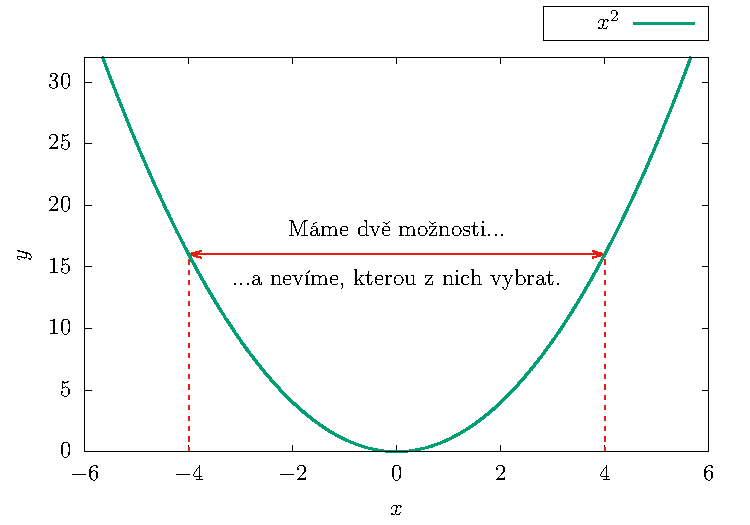
\includegraphics[scale = 0.7]{Gnuplot/cv1/Figures/nejednoznacny.pdf}
        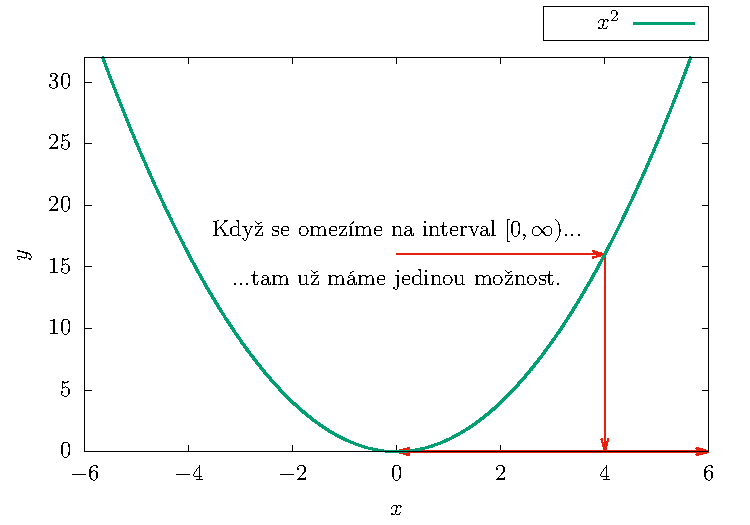
\includegraphics[scale = 0.7]{Gnuplot/cv1/Figures/nejednoznacny-reseni.pdf}
    \end{figure}

\end{example}

\begin{example}[Exponenciální funkce, přirozený logaritmus]
    Definujeme exponenciální funkci $\exp(x) = e^x$, kde $e = 2,718281828\cdots$ je tzv. Eulerovo číslo. (Je iracionální, stejně jako číslo $\pi$, číslice v desetinném zápisu se neopakují.) Dále definujeme funkci k ní inverzní - přirozený logaritmus $\ln(x) = \log_e (x)$. 
    Platí \begin{align}
        D(\exp(x)) = \R \:,\quad H(\exp(x)) = (0,+\infty) \:,\quad  D(\ln(x)) = (0,+\infty) \:,\quad  H(\ln(x)) = \R \:.
    \end{align}
    Užitečné vztahy, které se vyplatí pamatovat, jsou: \begin{align}
        e^0 = 1 \:,&\quad \ln(1) =0 \\
        e^{x+y} = e^x e^y \:,& \quad e^{ax} = (e^x)^a\\
        \ln(xy) = \ln x + \ln y \:,& \quad \ln(x^a) = a \ln x 
    \end{align}
    Grafy obou funkcí jsou znázorněny na obrázku \ref{fig:exp-log}.

    \begin{figure}[H]
        \centering
        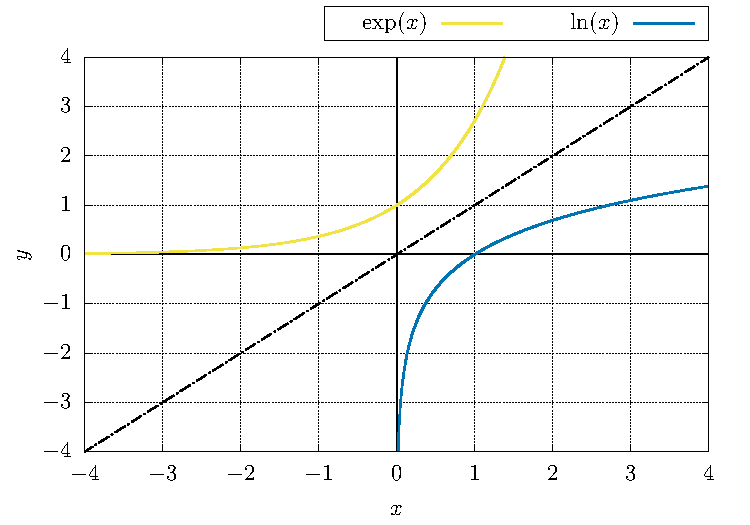
\includegraphics{Gnuplot/cv1/Figures/exp-log.pdf}
        \caption{Grafy funkcí exponenciály a přirozeného logaritmu. Všimněme si, že jsou grafy navzájem osově symetrické podle přímky $y=x$.}
        \label{fig:exp-log}
    \end{figure}

\end{example}
%\section*{Domácí úkol 1}
\textbf{Termín odevzdání:} na cvičení 7. nebo 8.10.2021.
\newline
\textbf{Zadání:} Cílem domácího úkolu je přesvědčit se, že platí \begin{align*}
    h(\mat A) = h(\mat A^T)  \:,
\end{align*}
kde $\mat A^T$ je transponovaná matice, která vznikne z matice $\mat A$ záměnou řádků za sloupce.

\begin{enumerate}
    \item \textbf{(0.5 bodu)} Sestavte matici $\mat A$ typu $4 \times 4$ takovou, že neobsahuje žádnou nulu a $h(\mat A) = 2$. 
    \item \textbf{(0.5 bodu)} Sestavte k ní transponovanou matici $\mat A^T$. Gaussovou eliminací určete její hodnost $h(\mat A^T)$. 
\end{enumerate}

Úkol odevzdejte, prosím, na papíře se svým jménem a časem cvičení, na které chodíte.
%\section*{Soustavy lineárních rovnic}

Soustavou $m$ lineárních rovnic o $n$ neznámých nazýváme rovnice tvaru
\begin{align}
    a_{11} x_1 + a_{12} x_2 + a_{13} x_3 + \cdots + a_{1n} x_n &= b_1 \:, \\
    a_{21} x_1 + a_{22} x_2 + a_{23} x_3 + \cdots + a_{2n} x_n &= b_2 \:, \\
    \vdots \\
    a_{m1} x_1 + a_{m2} x_2 + a_{m3} x_3 + \cdots + a_{mn} x_n &= b_m \:.
\end{align}
Seřadíme-li neznámé proměnné do vektoru $ \vc x = (x_1, x_2, \cdots, x_n) \in V_n$ a vytvoříme vektor z pravých stran \newline$\vc b = (b_1, b_2, \cdots, b_m) \in V_m$, můžeme soustavu napsat také v maticovém tvaru:
\begin{align}
    \mat A \vc x = \vc b \:.
\end{align}

\subsection*{Existence a počet řešení}

Definujeme matici soustavy \begin{align}
    \mat A = \begin{pmatrix}
        a_{11} & a_{12} & a_{13} & \cdots & a_{1n} \\
        a_{21} & a_{22} & a_{23} & \cdots & a_{2n} \\
        a_{31} & a_{32} & a_{33} & \cdots & a_{3n} \\
        \vdots & \vdots & \vdots & \ddots & \vdots \\
        a_{m1} & a_{m2} & a_{m3} & \cdots & a_{mn} 
    \end{pmatrix}
\end{align}
a rozšířenou matici soustavy \begin{align}
    \mat A_r = 
    \left(\begin{array}{ccccc|c}
        a_{11} & a_{12} & a_{13} & \cdots & a_{1n} & b_1\\
        a_{21} & a_{22} & a_{23} & \cdots & a_{2n} & b_2\\
        a_{31} & a_{32} & a_{33} & \cdots & a_{3n} & b_3\\
        \vdots & \vdots & \vdots & \ddots & \vdots & \vdots\\
        a_{m1} & a_{m2} & a_{m3} & \cdots & a_{mn} & b_m \\
        \end{array}\right) \:.
\end{align}

Klíčem k úspěchu je všimnout si, že elementární řádkové úpravy (eřú), které zachovávají hodnost matice, můžeme provádět i s rovnicemi: prohodit dvě rovnice zcela jistě můžeme, vynásobit rovnici nenulovým číslem také a součet dvou platných rovnic je rovněž platná rovnice. Můžeme tedy pracovat s maticemi, protože to je pohodlnější, a kdykoli je zpátky převádět na rovnice.

Pro určení počtu řešení soustavy se používají podmínky, které se ptají na hodnost obou těchto matic:
\begin{itemize}
    \item Jestliže $h(\mat A) \neq h(\mat A_r)$, pak soustava nemá žádné řešení.
    \item Jestliže $h(\mat A) = h(\mat A_r) = n$, pak má soustava právě jedno řešení.
    \item Jestliže $h(\mat A) = h(\mat A_r) < n$, pak má soustava nekonečně mnoho řešení. V takovém případě můžeme $n - h(\mat A)$ neznámých volit jako reálné parametry a zbylých $h(\mat A)$ neznámých dopočítáme.
\end{itemize}

\subsection*{Jediné řešení}

\begin{example}
    Uvažujme soustavu \begin{align}
        2x - y = 5 \:, \quad  x + 4y = -2 \:.
    \end{align}
    Napíšeme si rozšířenou matici soustavy:
    \begin{align}
       \mat A_r = \left( \begin{array}{rr|r}
            2 & -1 & 5 \\ 1 & 4 & -2
        \end{array}\right) \:.
    \end{align}
    Chtěli bychom určit hodnost. Tu určíme pomocí eřú převedením matice na odstupňovaný tvar:
    \begin{align}
        \left( \begin{array}{rr|r}
            2 & -1 & 5 \\ 1 & 4 & -2
        \end{array}\right)
        \sim
        \left( \begin{array}{rr|r}
            2 & -1 & 5 \\ -2 & -8 & 4
        \end{array}\right)
        \sim
        \left( \begin{array}{rr|r}
            2 & -1 & 5 \\ 0 & -9 & 9
        \end{array}\right) \:.
    \end{align}
    (V prvním kroku jsme druhý řádek vynásobili $-2$ a ve druhém kroku k němu přičetli první řádek.)
    Vidíme, že $h(\mat A) = h(\mat A_r) = 2$. Počet neznámých je rovněž $2$, proto má soustava právě jediné řešení.

    V odstupňovaném tvaru máme dvě rovnice 
    \begin{align}
        2x - y = 5 \:, \quad -9y = 9 \:.
    \end{align}
    Z druhé rovnice okamžitě vidíme $ y = -1$. Dosazením do první rovnice dostaneme $2x + 1 =5$, takže $x = 2$.

    Řešení můžeme zapsat ve vektorovém tvaru jako $\vc x = (2,-1)$.
\end{example}

\subsection*{Nekonečně mnoho řešení - jeden parametr}

\begin{example}
    Uvažujme soustavu \begin{align}
        x + 4y + 2z = 4 \:, \quad -3x+y+z=1 \:, \quad -x + 9y + 5z = 9 \:.
    \end{align}
    Sestavíme matici
    \begin{align}
       \mat B_r = \left( \begin{array}{rrr|r}
        1 & 4 & 2 & 4 \\ -3 & 1 & 1 & 1 \\ -1 & 9 & 5 & 9
    \end{array}\right) \:.
    \end{align}
    Opět ji pomocí eřú převedeme na odstupňovaný tvar:
    \begin{align}
        \left( \begin{array}{rrr|r}
            1 & 4 & 2 & 4 \\ -3 & 1 & 1 & 1 \\ -1 & 9 & 5 & 9
        \end{array}\right)
        \sim
        \left( \begin{array}{rrr|r}
            1 & 4 & 2 & 4 \\ 0 & 13 & 7 & 13 \\ 0 & 13 & 7 & 13
        \end{array}\right)
        \sim
        \left( \begin{array}{rrr|r}
        1 & 4 & 2 & 4 \\ 0 & 13 & 7 & 13 \\ 0 & 0 & 0 & 0
        \end{array}\right) \:.
    \end{align}
    (K druhému řádku jsme přičetli $3$-násobek prvního a ke třetímu první řádek.)

    Vidíme, že $h(\mat B) = h(\mat B_r) = 2 < 3$. Můžeme tedy volit $3-2 =1$ neznámých jako volitelné parametry. V našem případě můžeme jednu z proměnných volit jako libovolné reálné číslo, např. tu poslední:
    \begin{align}
        z = t \in \R \:.
    \end{align}
    Druhá rovnice nám dává $13y + 7t = 13$, odtud
    \begin{align}
        y = 1 - \frac{7}{13} t \:.
    \end{align}
    První rovnice nám říká $x + 4y + 2z = 4$, po dosazení \begin{align}
        x + 4 \left( 1 - \frac{7}{13} t \right) + 2t = 4 \:, 
    \end{align}
    odtud
    \begin{align}
        x = \frac{2}{13} t \:.
    \end{align}

    Proměnné $x$ a $y$ jsme tedy vyjádřili pomocí reálného parametru $t$. Řešení můžeme zapsat ve vektorovém tvaru. Pro přehlednost rozdělujeme řešení na konstantní část, která na žádném parametru nezávisí, a na proměnnou část, která je násobkem daného parametru. Zde
    \begin{align}
        \vc x = \left( \frac{2}{13} t , 1 - \frac{7}{13}, t \right) = \left( 0, 1, 0 \right) + ( \frac{2}{13}, -\frac{7}{13} , 1 ) \cdot t \:.
    \end{align}

\end{example}

\subsection*{Žádné řešení}

\begin{example}
    Uvažujme soustavu 
    \begin{align}
        x_1 - 4 x_2 + 2x_3 = 1 \:, \quad 3 x_1 - 7 x_2 + x_3 - 5 x_4 = -6 \:, \\
        x_2 - x_3 - x_4 = -1 \:, \quad 2 x_1 - 3 x_2 - x_3 - 5 x_4 = -7 \:.
    \end{align}
    Matice soustavy je
    \begin{align}
        \mat D_r = \left( \begin{array}{rrrr|r}
            1 & -4 & 2 & 0 & 1 \\ 3 & -7 & 1 & -5 & -6 \\ 0 & 1& -1 & -1 & -1 \\ 2 & -3 & -1 & -5 & -7 
        \end{array}\right)
    \end{align}
    Opět převádíme na odstupňovaný tvar:
    \begin{align}
        \left( \begin{array}{rrrr|r}
            1 & -4 & 2 & 0 & 1 \\ 3 & -7 & 1 & -5 & -6 \\ 0 & 1& -1 & -1 & -1 \\ 2 & -3 & -1 & -5 & -7 
        \end{array}\right)
        \sim
        \left( \begin{array}{rrrr|r}
            1 & -4 & 2 & 0 & 0 \\ 0 & 5 & -5 & -5 & -9 \\ 0 & 1& -1 & -1 & -1 \\ 0 & 5 & -5 & -5 & -9 
        \end{array}\right)
        \sim
        \left( \begin{array}{rrrr|r}
            1 & -4 & 2 & 0 & 0 \\ 0 & 5 & -5 & -5 & -9 \\ 0 & 0 & 0 & 0 & -4 \\ 0 & 0 & 0 & 0 & 0
        \end{array}\right) \:.
    \end{align}
    Vidíme, že $h(\mat D) = 2$, ale $h(\mat D_r) = 3$. Tato soustava tedy nemá žádné řešení.

    Proč tomu tak je? Třetí řádek nám vlastně dává rovnici $0x_1 + 0x_2 + 0x_3 + 0x_4 = -4$. Takovou rovnici nikdy nebudeme schopni splnit. To nám říká, že jedna z původních rovnic \uv{je tam navíc}, nemůžeme ji splnit nikdy.
\end{example}

\subsection*{Nekonečně mnoho řešení - více parametrů}

\begin{example}
    Řešme soustavu
    \begin{align}
        x_1 + x_2 + x_3 - x_4 - 2x_5 = 4 \:, \quad x_1 - x_3 + 2 x_4 = 0 \:.
    \end{align}
    Sestavíme matici
    \begin{align}
        \mat C_r = \left(\begin{array}{rrrrr|r}
            1 & 1 & 1 & -1 &-2 &4 \\ 1 &0 &-1 &2 &0 &0 
        \end{array}\right)
    \end{align}
    a dál to známe:
    \begin{align}
        \left(\begin{array}{rrrrr|r}
            1 & 1 & 1 & -1 &-2 &4 \\ 1 &0 &-1 &2 &0 &0 
        \end{array}\right)
        \sim
        \left(\begin{array}{rrrrr|r}
            1 & 1 & 1 & -1 &-2 &4 \\ 0 &1 &2 &-3 &-2 & 4 
        \end{array}\right)
    \end{align}
    Zde jsme druhý řádek vynásobili $-1$ a přičetli k němu první řádek. Platí $h(\mat C) = h(\mat C_r) = 2 < 5$, máme tedy k dispozici $5-2=3$ parametrů, které můžeme volit.
    
    \underline{Při volbě více parametrů postupujme odzadu.} Označme tedy
    \begin{align}
        x_5 = t_5 \in \R \:, x_4 = t_4 \in \R :, x_3 = t_3 \in \R \:.
    \end{align}
    Druhá rovnice říká \begin{align}
        x_2 + 2 t_3 - 3 t_4 - 2 t_5 = 4 \implies x_2 = 4 - 2 t_3 + 3 t_4 + 2 t_5 \:.
    \end{align}
    První rovnice říká \begin{align}
        x_1 + (4 - 2 t_3 + 3 t_4 + 2 t_5) + t_3 - t_4 - 2 t_5 = 4 \implies x_1 = t_3 - 2t_4 \:.
    \end{align}

    Nyní už je snad lépe vidět výhoda vektorového zápisu, který rozdělíme na čtyři části:
    \begin{align}
        \vc x = (0,4,0,0,0) + (1,-2,1,0,0) t_3 + (-2,3,0,1,0) t_4 + (0,2,0,0,1) t_5 \:.
    \end{align}
\end{example}

\subsection*{Dodatek: jaké proměnné mohou býti volitelné?}

\begin{example}
    Uvažujme soustavu (napišme ji rovnou v maticovém tvaru)
    \begin{align}
        \mat K_r = \left(\begin{array}{rrrrrrrrr|r}
            x_1 & x_2 & x_3 & x_4 & x_5 & x_6 & x_7 & x_8 & x_9 \\ \hline
            1 & 2 & -1 & 0 & 3 & 4 & 5 & 6 & 4 & 2 \\
            0 & 0 & 2  & -1 & 1 & 1 & 2 & -1 & 0 & 1 \\
            0 & 0 & 0  & 0 & 0 & 0 & 1 & 1 & 2 & 4 \\
        \end{array}\right) \:.
    \end{align}
    Hodnost matice $\mat K = \mat K_r = 3$, máme k dispozici $9-3=6$ volitelných parametrů. Jak je vybrat? Stačí se řídit dvěma zásadami:
    \begin{itemize}
        \item Jako parametry volíme proměnné postupně \uv{směrem odzadu}. 
        \item V jednom řádku (rovnici) nemohou vystupovat samé volitelné proměnné. První nenulové číslo tedy musí příslušet závislé proměnné.
    \end{itemize}
    Podívejme se na třetí řádek. To je rovnice \begin{align}
        x_7 + x_8 + 2x_9 = 4 \:.
    \end{align}
    Postupujeme směrem odzadu a označíme volitelné parametry $x_9 = t_9 \in \R$, $x_8 = t_8 \in \R$. Nemůžeme ovšem jako volitelný parametr označit $x_7$, protože pak bychom dostali rovnici
    \begin{align}
        t_7 + t_8 + 2t_9 = 4 \:,
    \end{align}
    která zjevně nemůže být splněna pro všechna reálná čísla! Z toho plyne, že $x_7$ musí být závislé na $t_8$ a $t_9$, konkrétně
    \begin{align}
        x_7 = 4 - t_8 - 2 t_9 \:.
    \end{align}
    Teď se podívejme na druhý řádek, který říká:
    \begin{align}
        2 x_3 - x_4 + x_5 + x_6 + 2 (4 - t_8 - 2 t_9) -t_8  = 1 \:.
    \end{align}
    Řídíme se pravidlem a můžeme opět označit $x_6 = t_6 \in \R$, $x_5 = t_5 \in \R$, $x_4 = t_4 \in \R$. Ale opět nesmí být $x_3$ volitelné, protože bychom dostali rovnici se samými volitelnými parametry, která by nebyla platná.
    Úplně stejně v první rovnici označíme $x_2$ jako volitelnou proměnnou, ale $x_1$ musí být závislá proměnná. Situace je tedy následující (symbolem $\checkmark$ označuji proměnnou, kterou lze volit jako parametr, symbolem $\times$ proměnnou, která musí být závislá na ostatních):
    \begin{align}
        \left(\begin{array}{rrrrrrrrr|r}
            x_1 & x_2 & x_3 & x_4 & x_5 & x_6 & x_7 & x_8 & x_9 \\ \hline
            1 & 2 & -1 & 0 & 3 & 4 & 5 & 6 & 4 & 2 \\
            0 & 0 & 2  & -1 & 1 & 1 & 2 & -1 & 0 & 1 \\
            0 & 0 & 0  & 0 & 0 & 0 & 1 & 1 & 2 & 4 \\ \hline
            \times & \checkmark & \times & \checkmark & \checkmark & \checkmark & \times & \checkmark & \checkmark
        \end{array}\right) \:.
    \end{align}
\end{example}

\subsection*{Soustavy s parametry}

\begin{example}
    V závislosti na $\alpha, \beta$ určíme řešení soustavy rovnic \begin{align}
        x_1 + \alpha x_2 + x_3 = 4 \:, \quad x_1 + x_2 + 2 x_3 = 4 \:, x_1 + x_2 + \beta x_3 = 3 \:.
    \end{align}
    Soustavu přepíšeme do matice a určíme její hodnost převedením na odstupňovaný tvar:
    \begin{align}
        \left(\begin{array}{rrr|r}
            1 & \alpha & 1 & 4 \\ 1 & 1 & 2 & 4 \\ 1 & 1 & \beta & 3 
        \end{array}\right) 
        \sim
        \left(\begin{array}{rrr|r}
            1 & \alpha & 1 & 4 \\ 0 & \alpha - 1 & -1 & 0 \\ 0 & 0 & \beta - 2 & -1 
        \end{array}\right)
        \:.
    \end{align}
    Nyní musíme rozlišit případy, kdy budeme mít nějaký nulový člen na hlavní diagonále.

    \begin{itemize}
        \item Případ $\beta - 2 = 0$, tj $\beta = 2$: soustava má tvar
        \begin{align}
            \left(\begin{array}{rrr|r}
                1 & \alpha & 1 & 4 \\ 0 & \alpha - 1 & -1 & 0 \\ 0 & 0 & 0 & -1 
            \end{array}\right)
            \:,
        \end{align}
        takže hodnost původní a rozšířené matice jsou různé. Soustava nemá žádné řešení.

        \item Případ $\beta \neq 2$, $\alpha - 1 =0$, tj $\alpha = 1$: soustava má tvar
        \begin{align}
            \left(\begin{array}{rrr|r}
                1 & \alpha & 1 & 4 \\ 0 & 0 & -1 & 0 \\ 0 & 0 & \beta - 2 & -1 
            \end{array}\right)
            \sim
            \left(\begin{array}{rrr|r}
                1 & \alpha & 1 & 4 \\ 0 & 0 & -1 & 0 \\ 0 & 0 & 0 & -1 
            \end{array}\right) \:.
        \end{align}
        Opět vidíme, že hodnosti jsou různé, proto soustava nemá žádné řešení.
        
        \item Případ $\beta \neq 2$, $\alpha \neq 1$. Nyní soustava nemá nuly na diagonále a je ve tvaru
        \begin{align}
            \left(\begin{array}{rrr|r}
                1 & \alpha & 1 & 4 \\ 0 & \alpha - 1 & -1 & 0 \\ 0 & 0 & \beta - 2 & -1 
            \end{array}\right)
            \:.
        \end{align}
        Hodnost původní a rozšířené matice jsou stejné a jsou stejné jako počet neznámých, máme proto jediné řešení. To snadno určíme. Třetí řádek nám říká
        \begin{align}
            (\beta - 2 ) x_3 = -1 \implies x_3 = - \frac{1}{\beta - 2} \:.
        \end{align}
        Druhý řádek říká
        \begin{align}
            (\alpha - 1 ) x_2 + \frac{1}{\beta - 2} = 0 \implies x_2 = - \frac{1}{(\alpha - 1)(\beta - 2)} \:.
        \end{align}
        První řádek Je
        \begin{align}
            x_1 - \frac{\alpha}{(\alpha - 1)(\beta - 2)} - \frac{4}{\beta - 2} = 4
            \implies x_1 = 4 + \frac{\alpha}{(\alpha - 1)(\beta - 2)} + \frac{4}{\beta - 2} \:.
        \end{align}
        Povšimněme si, že nulou v tomto případě nikdy nedělíme, protože tyto speciální případy jsme právě vyřešili výše.
    \end{itemize}

    Závěr: pro $\beta = 2$ anebo $\alpha = 1$ nemá soustava řešení. Pro $\alpha \neq 1$ a $\beta \neq 2$ má soustava jediné řešení.
\end{example}

\subsection*{Homogenní soustavy}

\textbf{Homogenní soustavy} jsou ve tvaru
\begin{align}
    a_{11} x_1 + a_{12} x_2  + \cdots + a_{1n} x_n &= 0 \:, \\
    a_{21} x_1 + a_{22} x_2  + \cdots + a_{2n} x_n &= 0 \:, \\
    \vdots \\
    a_{m1} x_1 + a_{m2} x_2  + \cdots + a_{mn} x_n &= 0 \:.
\end{align}

Takové soustavě přísluší matice s nulovým sloupcem pravé strany \begin{align}
    \mat A_r = \left( \mat A | \vc 0 \right) \:.
\end{align}
Hodnost matice se nezmění, přidáme-li k ní nulový sloupec, proto je vždy splněna podmínka $h(\mat A) = h(\mat A_r)$. Soustava má vždy řešení - je to řešení ze samých nul! Řešení ve tvaru $\vc x = \vc 0$ se nazývá \textbf{triviální řešení}. Samozřejmě nemusí být jediné, to bychom opět určili pomocí $h(\mat A)$.


\subsection*{Závěrečné poznámky}
\begin{itemize}
    \item Postup, který provádíme při řešení rovnic pomocí matic, se nazývá \textbf{Gaussova eliminace}.
    \item Drobnou modifikací tohoto postupu je \textbf{Jordanova metoda}, která spočívá v tom, že po převedení matice na odstupňovaný tvar se ji ještě snažíme vynulovat nad diagonálou, opět pomocí eřú. Získáme tak diagonální matici (kterou můžeme ještě převést na jednotkovou) a z ní můžeme přímo určit hodnoty neznámých. Protože je ale časově náročná, pro praktické počítání soustav se jí nepoužívá, bohatě si vystačíme s Gaussovou eliminací.
    \item Gaussova eliminace je praktická pro počítání na papíře, pokud chceme znát hodnoty všech neznámých proměnných. Seznámíme se později ještě s Cramerovým pravidlem, které je praktičtější v situacích, kdy nám stačí znát jenom některé neznámé, ale nepotřebujeme všechny.
\end{itemize}
%\section*{Násobení matic}

Matice $\mat A$ typu $n \times m$ a $\mat B$ typu $m \times k$ lze spolu vynásobit. Výsledná matice $\mat A \mat B$ je typu $n \times k$ a získáme ji pomocí pravidla \uv{řádek na sloupec}.

\begin{example}[Násobení pomocí tabulky]
    Nechť
    \begin{align}
        \mat A = \begin{pmatrix}
            2 & 4 & -1 & 0 \\
            1 & 0 & 3 & -2
        \end{pmatrix}
        \:, \quad
        \mat B = \begin{pmatrix}
            -1 & 1 & 2 \\
            3 & 0 & 0 \\
            1 & -2 & -1 \\
            -4 & 1 & 0 \\
        \end{pmatrix} \:.
    \end{align}
    Matice můžeme vynásobit pomocí pravidla řádek na sloupec. Výsledná matice bude zřejmě typu $2 \times 3$. Zápis, který může být užitečný, je sepsat si do tabulky \textbf{vlevo první matici} a \textbf{nahoru druhou matici}:
    \begin{align}
        \begin{array}{rrrr|rrr}
            &&&&-1 & 1 & 2 \\
            &&&&3 & 0 & 0 \\
            &&&&1 & -2 & -1 \\
            &&&&-4 & 1 & 0 \\
            \hline
            2 & 4 & -1 & 0 &     9 & 4 & 5\\
            1 & 0 & 3 & -2 &     10 & -7 & -1\\
        \end{array}
    \end{align}
    Například člen $1,1$ jsme získali součtem součinů: 
    \begin{align}
        2 \cdot (-1) + 4 \cdot 3 + (-1) \cdot 1 + 0 \cdot (-4) = 9 \:.
    \end{align}
    Takže \begin{align}
        \mat A \mat B = \begin{pmatrix}
            9 & 4 & 5 \\
            10 & -7 & -5
        \end{pmatrix} \:.
    \end{align}
    Matice v opačném pořadí vůbec vynásobit nelze, protože by neseděly rozměry.
\end{example}

\begin{example}[Nekomutativita matic]
    Ačkoli například čtvercové matice $\mat A$ a $\mat B$ můžeme násobit v obou směrech, neplatí, že by $\mat A \mat B$ a $\mat B \mat A$ byly stejné matice!
    Například \begin{align}
        \begin{pmatrix}
            1 & -1 \\
            0 & 2
        \end{pmatrix}
        \begin{pmatrix}
            -1 & -1 \\
            1 & 4
        \end{pmatrix}
        =
        \begin{pmatrix}
            -2 & -5 \\
            2 & 8
        \end{pmatrix} \:, \quad
        \begin{pmatrix}
            -1 & -1 \\
            1 & 4
        \end{pmatrix}
        \begin{pmatrix}
            1 & -1 \\
            0 & 2
        \end{pmatrix}
        =
        \begin{pmatrix}
            -1 & -1\\
            1 & 7\\
        \end{pmatrix} \:.
    \end{align}

    Přesvědčte se sami, že násobit v obou směrech lze i matice typu $m \times n$ a $n \times m$. Rozměr výsledné matice ale bude pokaždé jiný!

    \underline{Musíme proto přísně rozlišovat mezi násobením matic zleva a zprava.}
\end{example}

Pro násobení matic platí
\begin{itemize}
    \item \textbf{nekomutativita}: $\mat A \mat B \neq \mat B \mat A$
    \item \textbf{asociativita}: $\mat A (\mat B \mat C) = (\mat A \mat B) \mat C$
    \item \textbf{distributivita} (zprava a zleva): $(\mat A + \mat B) \mat C = \mat A \mat C + \mat B \mat C$, $\mat A(\mat B + \mat C) = \mat A \mat B + \mat A \mat C$
\end{itemize}

\section*{Inverzní matice}

Čtvercové matice typu $n \times n$ označujeme jako matice řádu $n$.

Definujeme \textbf{jednotkovou matici} $\mat J$ řádu $n$ (v literatuře se pro ni používá též značení $\mat E$, $\mat I$, $\mat E_n$, $\mat{Id}$) jako čtvercovou matici řádu $n$, která má na hlavní diagonále samé jedničky a jinde nuly. Je-li $\mat A$ čtvercová matice řádu $n$, pak zjevně platí $\mat A \mat J = \mat J \mat A = \mat A$.

\textbf{Inverzní matice} $\mat A^{-1}$ je čtvercová matice stejného řádu $n$, která splňuje $\mat A \mat A^{-1} = \mat A^{-1} \mat A = \mat J$. Pokud inverzní matice existuje, je definována jednoznačně. Není ale definována pro všechny čtvercové matice. 

Řekneme, že matice $\mat A$ řádu $n$ je \textbf{regulární}, jestliže $h(\mat A) = n$, v opačném případě řekneme, že je \textbf{singulární}. Pouze pro regulární matice existuje matice inverzní.

\subsection*{Hledání inverzní matice Jordanovou metodou}

Pro výpočet inverzní matice lze použít metodu, kterou jsme zmiňovali u řešení soustavy lineárních rovnic. Matici $\mat A$ rozšíříme o jednotkovou matici $\mat J$ a pomocí elementárních řádkových úprav se ji pokusíme převést na tvar, kde bude na levé straně vystupovat jednotková matice $\mat J$. Na pravé straně pak získáme inverzní matici $\mat A^{-1}$.
\begin{align}
    (\mat A | \mat J) \rightarrow \text{eřú} \rightarrow (\mat J | \mat A^{-1})
\end{align}

\begin{example}
    Určíme inverzní matici k \begin{align}
        \mat B = \begin{pmatrix}
            1 & -1 & 0 \\
            2 & 0 & 1 \\
            -1 & -1 & 4
        \end{pmatrix} \:.
    \end{align}
    Tato matice má $h(\mat B ) = 3$, je proto regulární a inverzní matice k ní existuje.
    Napíšeme si tvar \begin{align}
        (\mat B | \mat J) = \left(\begin{array}{rrr|rrr}
            1 & -1 & 0 & 1 & 0 & 0\\
            2 & 0 & 1 & 0 & 1 & 0\\
            -1 & -1 & 4 & 0 & 0 & 1
        \end{array}\right) \:.
    \end{align}
    Nyní začneme provádět eřú. Nejprve se snažíme vynulovat členy pod diagonálou, stejně jako u Gaussovy eliminace. Začneme standartně prvním sloupcem a pokračovat budeme druhým sloupcem.
    \begin{align}
        \left(\begin{array}{rrr|rrr}
            1 & -1 & 0 & 1 & 0 & 0\\
            2 & 0 & 1 & 0 & 1 & 0\\
            -1 & -1 & 4 & 0 & 0 & 1
        \end{array}\right) 
        \sim
        \left(\begin{array}{rrr|rrr}
            1 & -1 & 0 & 1 & 0 & 0\\
            0 & 2 & 1 & -2 & 1 & 0\\
            0 & -2 & 4 & 1 & 0 & 1
        \end{array}\right)
        \sim
        \left(\begin{array}{rrr|rrr}
            1 & -1 & 0 & 1 & 0 & 0\\
            0 & 2 & 1 & -2 & 1 & 0\\
            0 & 0 & 5 & -1 & 1 & 1
        \end{array}\right) \:.
    \end{align}
    Nyní chceme vynulovat členy nad diagonálou. Začneme posledním sloupcem a pokračovat budeme prostředním. Poslední řádek rovnou vydělíme pěti.
    \begin{align}
        \left(\begin{array}{rrr|rrr}
            1 & -1 & 0 & 1 & 0 & 0\\
            0 & 2 & 1 & -2 & 1 & 0\\
            0 & 0 & 5 & -1 & 1 & 1
        \end{array}\right)
        \sim&
        \left(\begin{array}{rrr|rrr}
            1 & -1 & 0 & 1 & 0 & 0\\
            0 & 2 & 0 & -2+\frac{1}{5} & 1-\frac{1}{5} & -\frac{1}{5}\\
            0 & 0 & 1 & -\frac{1}{5} & \frac{1}{5} & \frac{1}{5}
        \end{array}\right)
        \sim
        \left(\begin{array}{rrr|rrr}
            1 & -1 & 0 & 1 & 0 & 0\\
            0 & 1 & 0 & -\frac{9}{10} & \frac{4}{10} & -\frac{1}{10}\\
            0 & 0 & 1 & -\frac{1}{5} & \frac{1}{5} & \frac{1}{5}
        \end{array}\right)
        \sim \\ \sim&
        \left(\begin{array}{rrr|rrr}
            1 & 0 & 0 & 1-\frac{9}{10} & \frac{4}{10} & -\frac{1}{10}\\
            0 & 1 & 0 & -\frac{9}{10} & \frac{4}{10} & -\frac{1}{10}\\
            0 & 0 & 1 & -\frac{1}{5} & \frac{1}{5} & \frac{1}{5}
        \end{array}\right)
        \sim
        \left(\begin{array}{rrr|rrr}
            1 & 0 & 0 & \frac{1}{10} & \frac{4}{10} & -\frac{1}{10}\\
            0 & 1 & 0 & -\frac{9}{10} & \frac{4}{10} & -\frac{1}{10}\\
            0 & 0 & 1 & -\frac{2}{10} & \frac{2}{10} & \frac{2}{10}
        \end{array}\right) \:.
    \end{align}
    Nalevo máme jednotkovou matici. Napravo jsme získali matici inverzní:
    \begin{align}
        \mat B^{-1} = \begin{pmatrix}
            \frac{1}{10} & \frac{4}{10} & -\frac{1}{10}\\
            -\frac{9}{10} & \frac{4}{10} & -\frac{1}{10}\\
            -\frac{2}{10} & \frac{2}{10} & \frac{2}{10}
        \end{pmatrix}
        = \frac{1}{10} \begin{pmatrix}
            1 & 4 & -1 \\
            -9 & 4 & -1 \\
            -2 & 2 & 2
        \end{pmatrix}
    \end{align}

    Můžeme se přesvědčit o tom, že je to správná inverzní matice:
    \begin{align}
        \mat B \mat B^{-1} = \frac{1}{10} \begin{pmatrix}
            1 & -1 & 0 \\
            2 & 0 & 1 \\
            -1 & -1 & 4
        \end{pmatrix} \begin{pmatrix}
            1 & 4 & -1 \\
            -9 & 4 & -1 \\
            -2 & 2 & 2
        \end{pmatrix}
        =
        \frac{1}{10}
        \begin{pmatrix}
            10 & 0 & 0 \\ 0 & 10 & 0 \\ 0 & 0 & 10
        \end{pmatrix}
        = \mat J
    \end{align}
    a obdobně v opačném pořadí.
\end{example}

\begin{example}
    Matice \begin{align}
        \mat M = \begin{pmatrix}
            4 & 2 \\
            -2 & -1
        \end{pmatrix}
    \end{align}
    nemá k sobě inverzní, protože $h(\mat M) = 1$. Pokud bychom se pokusili hledat ji Jordanovou metodou, narazili bychom na potíže:
    \begin{align}
        \left(\begin{array}{rr|rr}
            4 & 2 & 1 & 0\\
            -2 & -1 & 0 & 1
        \end{array}\right)
        \sim
        \left(\begin{array}{rr|rr}
            4 & 2 & 1 & 0\\
            0 & 0 & 1 & 2
        \end{array}\right) \:.
    \end{align}
    Na levé straně se nám žádným způsobem nepovede vynulovat dvojku nad diagonálou.
\end{example}

\subsection*{Poznámky}

\begin{itemize}
    \item Asi nejsnáze se určuje regularita/singularita matice pomocí determinantu.
    \item K hledání inverzní matice řádu 2 se používá často triku, který je v českých zemích pojmenován \uv{Čihákovo pravidlo} na počest profesora Čiháka, který přednášel dlouhá léta na MATFYZu. Seznámíme se s ním v jednom pozdějším domácím úkolu.
    \item Další vlastnost maticové algebry je, že $(\mat A \mat B)^{-1} \neq \mat A^{-1} \mat B^{-1}$. Ve skutečnosti $(\mat A \mat B)^{-1} = \mat B^{-1} \mat A^{-1}$, což si ověříme rovněž v domácím úkolu.
    \item Stejně tak platí $(\mat A \mat B)^T = \mat B^T \mat A^T$.
\end{itemize}
%\section*{Domácí úkol 2}
\textbf{Termín odevzdání:} na cvičení 21. nebo 22.10.2021.
\newline
\textbf{Zadání:} Cílem domácího úkolu je přesvědčit se o identitě tvaru \begin{align*}
    (\mat A \mat B)^{-1} = \mat B^{-1} \mat A^{-1} \:.
\end{align*}

\begin{itemize}
    \item \textbf{(0.25 bodu)} Vymyslete dvě \uv{netriviální} regulární matice $\mat A$, $\mat B$ řádu $2$.
    \item \textbf{(0.25 bodu)} Spočtěte jejich inverzní matice $\mat A^{-1}$, $\mat B^{-1}$.
    \item \textbf{(0.25 bodu)} Spočtěte součin $\mat C = \mat B^{-1} \mat A^{-1}$.
    \item \textbf{(0.25 bodu)} Spočtěte součin $\mat D = \mat A \mat B$ a k této matici sestrojte inverzní $\mat D^{-1}$. \newline(Výsledné matice by si měly odpovídat: $\mat C = \mat D^{-1}$)
\end{itemize}

\textbf{Poznámka:} Z identity je vidět, že součin dvou regulárních matic bude opět regulární matice (protože k takovému součinu existuje inverzní matice). Povšimněte si také, že $(\mat A \mat B)^{-1} \neq \mat A^{-1} \mat B^{-1}$.
\section*{Maticové rovnice}

\begin{example}
    Řešme rovnici
    \begin{align}
        \mat X \mat A - \mat B = 2 \mat X + \mat J \:,
        \quad \text{kde} \:
        \mat A = \begin{pmatrix}
            5 & 5 \\ 1 & 4 
        \end{pmatrix} \:,\:
        \mat B = \begin{pmatrix}
            0 & 1 \\ 3 & 2 
        \end{pmatrix} \:,\: \mat X \text{ je neznámá}\:.
    \end{align}
    Postupujeme podobně, jako bychom řešili obyčejnou lineární rovnici. Musíme však dbát na to, že násobené matic není komutativní - musíme rozlišovat násobení rovnic zprava a zleva.

    V prvním kroku přesuneme všechny $\mat X$ na levou stranu:
    \begin{align}
        \mat X \mat A - 2 \mat X = \mat J + \mat B \:. 
    \end{align}
    Symbol $2 \mat X$ lze také číst jako $\mat X \cdot 2 \mat J$. Můžeme proto vytknout před závorku $\mat X$:
    \begin{align}
        \mat X (\mat A - 2 \mat J) = \mat J + \mat B \:.
    \end{align}
    Jestliže existuje matice $(\mat A - 2 \mat J)^{-1}$, mohli bychom touto maticí vynásobit celou rovnici zprava:
    \begin{align}
        \mat X (\mat A - 2 \mat J)(\mat A - 2 \mat J)^{-1} = (\mat J + \mat B)(\mat A - 2 \mat J)^{-1}
    \end{align}
    a dostaneme řešení
    \begin{align}
        \mat X = (\mat J + \mat B)(\mat A - 2 \mat J)^{-1} \:.
    \end{align}

    Spočítejme tedy matici $\mat A - 2 \mat J$:
    \begin{align}
        \mat A - 2 \mat J = \begin{pmatrix}
            5 & 5 \\ 1 & 4 
        \end{pmatrix} - 2 \begin{pmatrix}
            1 & 0 \\ 0 & 1
        \end{pmatrix}
        =
        \begin{pmatrix}
            3 & 5 \\ 1 & 2
        \end{pmatrix} \:.
    \end{align}
    Tato matice je regulární, proto k ní můžeme inverzi najít. To učiníme Jordanovou metodou:
    \begin{align}
        \left(\begin{array}{cc|cc}
            3 & 5 & 1 & 0 \\
            1 & 2 & 0 & 1
        \end{array}\right)
        \sim
        \left(\begin{array}{cc|cc}
            3 & 5 & 1 & 0 \\
            0 & -1 & 1 & -3
        \end{array}\right)
        \sim
        \left(\begin{array}{cc|cc}
            3 & 0 & 6 & -15 \\
            0 & 1 & -1 & 3
        \end{array}\right)
        \sim
        \left(\begin{array}{cc|cc}
            1 & 0 & 2 & -5 \\
            0 & 1 & -1 & 3
        \end{array}\right)
    \end{align}
    Takže \begin{align}
        (\mat A - 2 \mat J)^{-1} = \begin{pmatrix}
            2 & -5 \\
            -1 & 3
        \end{pmatrix} \:.
    \end{align}
    Nyní už řešení najdeme jednoduchým násobením:
    \begin{align}
        \mat X = \left[
            \begin{pmatrix}
            1 & 0 \\ 0 & 1
            \end{pmatrix} 
        +
            \begin{pmatrix}
                0 & 1 \\ 3 & 2
            \end{pmatrix}    
        \right] \begin{pmatrix}
            2 & -5 \\ -1 & 3
        \end{pmatrix}
        = \begin{pmatrix}
            1 & 1 \\ 3 & 3
        \end{pmatrix}
        \begin{pmatrix}
            2 & -5 \\ -1 & 3
        \end{pmatrix}
        =
        \begin{pmatrix}
            1 & -2 \\ 3 & -6
        \end{pmatrix} \:.
    \end{align}
\end{example}

\begin{example}
    Řešme maticovou rovnici \begin{align}
        2 \mat X \mat K = \mat X + \mat B \:, \quad \text{kde} \: 
        \mat K = \begin{pmatrix}
            2 & 2 \\ -1 & -1
        \end{pmatrix} \:,
        \:
        \mat B = \begin{pmatrix}
            0 & 3 \\ 0 & -2
        \end{pmatrix} \:.
    \end{align}
    Ukážeme si alternativní způsob řešení takové rovnice. Tento způsob se používá hlavně v případě, když narazíme na součin neznámé matice s jinou, která není regulární, a nemá proto inverzi. Tento postup lze použít vždy, ale je trochu časově náročnější.
    
    Rozepíšeme si neznámou matici $\mat X$ do složek a budeme hledat rovnice pro jednotlivé složky (označíme je postupně):
    \begin{align}
        \mat X = \begin{pmatrix}
            x_1 & x_2 \\ x_3 & x_4
        \end{pmatrix} \:.
    \end{align}
    Dostáváme rovnici
    \begin{align}
        2
        \begin{pmatrix}
            x_1 & x_2 \\ x_3 & x_4
        \end{pmatrix}
        \begin{pmatrix}
            2 & 2 \\ -1 & -1
        \end{pmatrix}
        =
        \begin{pmatrix}
            x_1 & x_2 \\ x_3 & x_4
        \end{pmatrix}
        +
        \begin{pmatrix}
            0 & 3 \\ 0 & -2
        \end{pmatrix}
        \:.
    \end{align}
    Spočítáme levou stranu:
    \begin{align}
        \begin{pmatrix}
            4 x_1 - 2 x_2 & 4 x_1 - 2 x_2 \\ 4 x_3 - 2 x_4 & 4 x_3 - 2 x_4
        \end{pmatrix} 
        =
        \begin{pmatrix}
            x_1 & x_2 \\ x_3 & x_4
        \end{pmatrix}
        +
        \begin{pmatrix}
            0 & 3 \\ 0 & -2
        \end{pmatrix}
    \end{align}
    a odečteme první matici na pravé straně
    \begin{align}
        \begin{pmatrix}
            3 x_1 - 2 x_2 & 4 x_1 - 3 x_2 \\ 3 x_3 - 2 x_4 & 4 x_3 - 3 x_4
        \end{pmatrix}
        =
        \begin{pmatrix}
            0 & 3 \\ 0 & -2
        \end{pmatrix} \:.
    \end{align}
    To je ekvivalentní soustavě rovnic
        \begin{align}
            3 x_1 - 2 x_2 = 0 \:,\quad
            4 x_1 - 3 x_2 = 3 \:,\quad
            3 x_3 - 2 x_4 = 0 \:,\quad
            4 x_3 - 3 x_4 = -2 \:.
        \end{align}
    Tuto soustavu nyní vyřešíme standartně Gaussovou metodou.
    \begin{align}
        \left(\begin{array}{cccc|c}
            3 & -2 & 0 & 0 & 0 \\
            4 & -3 & 0 & 0 & 3 \\
            0 & 0 & 3 & -2 & 0 \\
            0 & 0 & 4 & -3 & -2 
        \end{array}\right)
        \sim
        \left(\begin{array}{cccc|c}
            12 & -8 & 0 & 0 & 0 \\
            -12 & 9 & 0 & 0 & -9 \\
            0 & 0 & 12 & -8 & 0 \\
            0 & 0 & -12 & 9 & 6 
        \end{array}\right)
        \sim
        \left(\begin{array}{cccc|c}
            12 & -8 & 0 & 0 & 0 \\
            0 & 1 & 0 & 0 & -9 \\
            0 & 0 & 12 & -8 & 0 \\
            0 & 0 & 0 & 1 & 6 
        \end{array}\right)
    \end{align}
    Takže vidíme, že $x_4 = 6$, $x_2 = -9$, dále máme dvě rovnice
    \begin{align}
        12 x_3 - 48 = 0 \implies x_3 = 4 \:, \quad 12 x_1 + 72 = 0 \implies x_1 = -6 \:.
    \end{align}
    Výsledná matice je rovna
    \begin{align}
        \mat X = \begin{pmatrix}
            -6 & -9 \\ 4 & 6
        \end{pmatrix} \:.
    \end{align}
    Můžeme se přesvědčit o správnosti: levá strana je
    \begin{align}
        \begin{pmatrix}
            -12 & -18 \\ 8 & 12
        \end{pmatrix}
        \begin{pmatrix}
            2 & 2 \\ -1 & -1 
        \end{pmatrix}
        =
        \begin{pmatrix}
            -6 & -6 \\ 4 & 4
        \end{pmatrix}
    \end{align}
    a pravá strana je \begin{align}
        \begin{pmatrix}
            -6 & -9 \\ 4 & 6
        \end{pmatrix}
        +
        \begin{pmatrix}
            0 & 3 \\ 0 & -2
        \end{pmatrix}
        =
        \begin{pmatrix}
            -6 & -6 \\ 4 & 4
        \end{pmatrix} \:,
    \end{align}
    takže všechno vychází.
\end{example}



\begin{example}
    Hledejme všechny matice, které komutují s maticí \begin{align}
        \mat F = \begin{pmatrix}
            0 & 2 \\ -2 & 0
        \end{pmatrix} \:.
    \end{align}
    Hledanou matici si označíme jako $\mat X$. Řešíme maticovou rovnici
    \begin{align}
        \mat X \mat F = \mat F \mat X \:.
    \end{align}
    Rozepišme si $\mat X$ do složek:
    \begin{align}
        \begin{pmatrix}
            x_1 & x_2 \\ x_3 & x_4
        \end{pmatrix}
        \begin{pmatrix}
            0 & 2 \\ -2 & 0
        \end{pmatrix}
        = 
        \begin{pmatrix}
            0 & 2 \\ -2 & 0
        \end{pmatrix}
        \begin{pmatrix}
            x_1 & x_2 \\ x_3 & x_4
        \end{pmatrix} \:.
    \end{align}
    Obě strany upravíme:
    \begin{align}
        \begin{pmatrix}
            -2x_2 & 2x_1 \\
            -2x_4 & 2x_3
        \end{pmatrix}
        =
        \begin{pmatrix}
            2x_3 & 2x_4 \\
            -2x_1 & -2x_2
        \end{pmatrix} \:.
    \end{align}
    Porovnáním jednotlivých složek dostáváme čtyři rovnice
    \begin{align}
        -2x_2 = 2x_3 \:,\quad 2x_1=2x_4 \:,\quad -2x_4=-2x_1 \:,\quad 2x_3=-2x_2
    \end{align}
    a hned vidíme, že nebude ani potřeba psát velké matice: dvě rovnice jsou identické a máme
    \begin{align}
        x_1 = x_4 = t \in \R \:, \quad -x_2 = x_3 = s \in \R \:,
    \end{align}
    takže
    \begin{align}
        \mat X = \begin{pmatrix}
            1 & 0 \\ 0 & 1
        \end{pmatrix} t
        +
        \begin{pmatrix}
            0 & -1 \\ 1 & 0
        \end{pmatrix} s \:.
    \end{align}
    (Výsledek je dosti intuitivní: s maticí komutují násobky jednotkové matice a násobky matice samotné.)
\end{example}

\subsection*{Řešení soustav lineárních rovnic pomocí inverzní matice}

Soustavu lineárních rovnic lze zapsat ve tvaru $\mat A \vc x = \vc b$, kde na $\vc x$ a $\vc b$ lze pohlížet jako na sloupcové vektory. Máme-li $n$ rovnic pro $n$ neznámých, jsou $\vc x \in V_n$, $\vc b \in V_n$ a matice $\mat A$ je řádu n. Jestliže je $\mat A$ regulární (její hodnost je $n$, tzn. má všechny řádky/sloupce lineárně nezávislé), pak můžeme rovnici vynásobit zleva maticí $\mat A^{-1}$ a dostáváme okamžitě řešení
\begin{align}
    \vc x = \mat A^{-1} \vc b \:.
\end{align}
Tento vztah platí, pokud matice $\mat A^{-1}$, to odpovídá případu, kdy má soustava právě jedno řešení. Pokud bychom měli soustavu s nekonečně mnoha řešeními nebo žádným řešením, pak by inverze neexistovala a rovnice by samozřejmě neplatila.

Protože hledání inverzní matice je v podstatě ekvivalentní Jordanově metodě, pro počítání na papíře se příliš nehodí. Užitečné je například v situacích, kdy máme více soustav se stejnou maticí $\mat A$ a rozdílnými vektory pravých stran $\vc b$.

\subsection*{Poznámky}
\begin{itemize}
    \item Maticové rovnice nemají velké uplatnění v praxi. Slouží hlavně k procvičování vlastností maticové algebry.
    \item Přestože spolu matice běžně nekomutují, existují velmi speciální třídy matic, které spolu komutují. Jednu takovou třídu jsme našli v příkladu výše. Takovým maticím se říká \textbf{normální} a mají velké uplatnění. Například mají zásadní úlohu v kvantové fyzice nebo v odvětví tzv. lineárního programování.
    \item Každá matice komutuje s jednotkovou maticí a sama se sebou (a samozřejmě s libovolnými násobky.)
    \item Jestliže matice $\mat A$ komutuje s $\mat B$ a současně i s $\mat C$, pak komutuje i s jejich součtem:
    \begin{align}
        \mat A (\mat B + \mat C) = \mat A \mat B + \mat A \mat C = \mat B \mat A + \mat C \mat A = (\mat B + \mat C) \mat A
    \end{align}
    i součinem:
    \begin{align}
        \mat A (\mat B \mat C) = (\mat A \mat B) \mat C = (\mat B \mat A) \mat C = \mat B (\mat A \mat C) = \mat B (\mat C \mat A) = (\mat B \mat C) \mat A \:. 
    \end{align}
    \item Matice $\mat A$ a $\mat A^T$ spolu běžně nekomutují.
\end{itemize}
\end{document}